
%%%%%%%%%%%%%%%%%%%%%%%%%%%%%%%%%%%%%%%%%%%%%%%%%%%%%%%%%%%%%%%%%%%%%%%%
%Para las ecuaciones siempre es Ec.(n).
%Para las figuras siempre es Fig.n, incluso en el caption de la figura. Tambien las Tablas
%Para las referencias es [n]
%%%%%%%%%%%%%%%%%%%%%%%%%%%%%%%%%%%%%%%%%%%%%%%%%%%%%%%%%%%%%%%%%%%%%%%%

\documentclass[
reprint,
%notitlepage,
%superscriptaddress,
%groupedaddress,
%unsortedaddress,
%runinaddress,
%frontmatterverbose, 
%preprint,
%showpacs,preprintnumbers,
%nofootinbib,
%nobibnotes,
%bibnotes,
%11 pt,
amsmath,
amssymb,
aps,
pra,
%prb,
%rmp,
%tightenlines %esto hizo el milagro de sacar los espacios en blancos estocásticos (?)
 %prstab,
%prstper,
%floatfix,\textbf{}
]{revtex4-1} %Instalar primero para usarlo. Paquete malo.

%\documentclass[onecolumn, aps, amsmath,amssymb ]{article}
\usepackage{lipsum}  
\usepackage{graphicx}% Include figure files
\usepackage{subfig}
\usepackage{braket}
\usepackage{comment} %comment large chunks of text
\usepackage{dcolumn}% Align table columns on decimal point
\usepackage{bm}% bold math
%\usepackage{hyperref}% add hypertext capabilities
\usepackage[mathlines]{lineno}% Enable numbering of text and display math
%\linenumbers\relax % Commence numbering lines
\usepackage{mathtools} %% Para el supraíndice

\usepackage[nice]{nicefrac}

%%%%%%%El Señor Español%%%%%%%%%%%%%%%%%%%%%%%%%%%
\usepackage[utf8]{inputenc} %acento
\usepackage[
spanish, %El lenguaje.
es-tabla, %La tabla y no cuadro.
activeacute, %El acento.
es-nodecimaldot %Punto y no coma con separador de números
]{babel}
\usepackage{microtype} %para hacerlo más bonito :33 como vos (?) 
%%%%%%%%%%%%%%%%%%%%%%%%%%%%%%%%%%%%%%%%%%%%%%%%%%%
%%%%%%%%% Para que las imágenes se queden dónde las quiero (?
\usepackage{float}
%%%%%%%%%%

%%%%%%%%Cambia a Fig de Figure%%%%%%%%%%
\makeatletter
\renewcommand{\fnum@figure}{Fig. \thefigure} 
\makeatother
%%%%%%%%%%%%%%%%%%%%%%%%%%%%%%%%%%%%%%%%
\raggedbottom

\usepackage{hyperref}
\usepackage{listings}
\usepackage{xcolor}


\definecolor{codegreen}{rgb}{0,0.6,0}
\definecolor{codegray}{rgb}{0.5,0.5,0.5}
\definecolor{codepurple}{rgb}{0.58,0,0.82}
\definecolor{backcolour}{rgb}{0.95,0.95,0.92}

%Code listing style named "mystyle"
\lstdefinestyle{mystyle}{
  backgroundcolor=\color{backcolour},   commentstyle=\color{codegreen},
  keywordstyle=\color{magenta},
  numberstyle=\tiny\color{codegray},
  stringstyle=\color{codepurple},
  basicstyle=\ttfamily\footnotesize,
  breakatwhitespace=false,         
  breaklines=true,                 
  captionpos=b,                    
  keepspaces=true,                 
  numbers=left,                    
  numbersep=5pt,                  
  showspaces=false,                
  showstringspaces=false,
  showtabs=false,                  
  tabsize=2
}
\lstset{style=mystyle}

\begin{document}
%%%%%%%%%%%%%%%%%%%%%%%%%%%%%%%%%%Título%%%%%%%%%%%%%%%%%%%%%%%%%%%%%%%%%%%%%%
%%%%%%%%%%%%%%%%%%%%%%%%%%%%%%%%%%%%%%%%%%%%%%%%%%%%%%%%%%%%%%%%%%%%%%%%%%%%%%

\title{Práctica 3: Estadística de trenes de spikes }
\author{Evelyn~G.~Coronel}

\affiliation{
Redes~Neuronales - Instituto~Balseiro\\}

\date[]{\lowercase{\today}} %%lw para lw, [] sin date

\begin{abstract}
Soluciones a los ejercicios de la práctica 3 de la materia de Redes Neuronales. En esta práctica se estudia la estadística de los resultados obtenidos para un experimento, donde se excita un receptor acústico de un saltamontes mediante un sonido.
\end{abstract} 
\maketitle
%%%%%%%%%%%%%%%%%%%%%%%%%%%%%%%%%%%%%%%%%%%%%%%%%%%%%%%%%%%%%%%%%%%%%%%%%%%%%%%%%%%
%\section*{Introducción}

\section*{Estímulo y Respuestas}


Se realizaron 128 pruebas o realizaciones  donde se midió la respuesta del receptor de un saltamontes  acústico ante el mismo estimulo. En la parte superior de la Fig.\ref{experimento} se muestra se presenta el estímulo al que fue sometido el receptor acústico del insecto. Este estímulo tiene una varianza de  $\sigma^2_{s}= 31.65\,$dB$^2$.  

En la parte inferior de la Fig.\ref{experimento} se muestra se muestran, como puntos azules, las respuestas a este estimulo en función del tiempo, la adquisición de datos se realizó en ventanas de $0.1\,$ms. La presencia del punto indica que se midió un spike para ese ventana de tiempo. 

Puede verse que existen ventanas de tiempo donde se midieron más spikes que en otros, por ejemplo, la franja blanca para $t \approx 400\,$ms se tienen menos spikes que para $t\approx 1000\,$ms.

\begin{figure}[H]
	\centering
	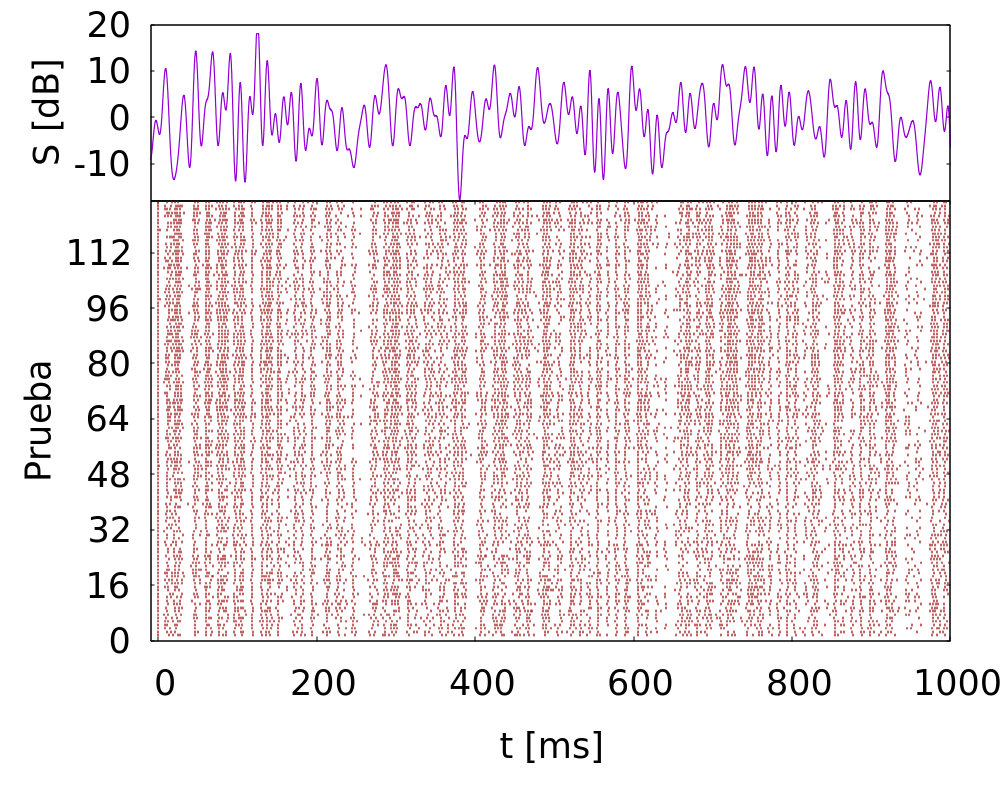
\includegraphics[width=0.45\textwidth]{../Graficos/stimulus.png}
	\caption{La figura superior representa la intensidad del estimulo en función de tiempo. La figura inferior representa todos los spikes observados en cada prueba.}
	\label{experimento}
\end{figure}


\section*{Distribución de intervalos \texorpdfstring{$P(\tau)$}{}}

Para cada prueba realizada, se calcula los intervalos de tiempo (ISI) entre dos spikes consecutivos, luego se calcula el histograma de estos valores como se muestra en la Fig.\,\ref{p_isi}. La distribución tiene una media de $\langle ISI \rangle = 85.198\,$ms y un varianza de $\sigma^2_{ISI}=3226.69\,$ms$^2$, mientras que el coeficiente de variabilidad es de $CV=0.659$. Se observa que existe un pico para $2.5\,$ms, esto puede indicar algo proceso característico del funcionamiento del receptor.

\begin{figure}[H]
	\centering
	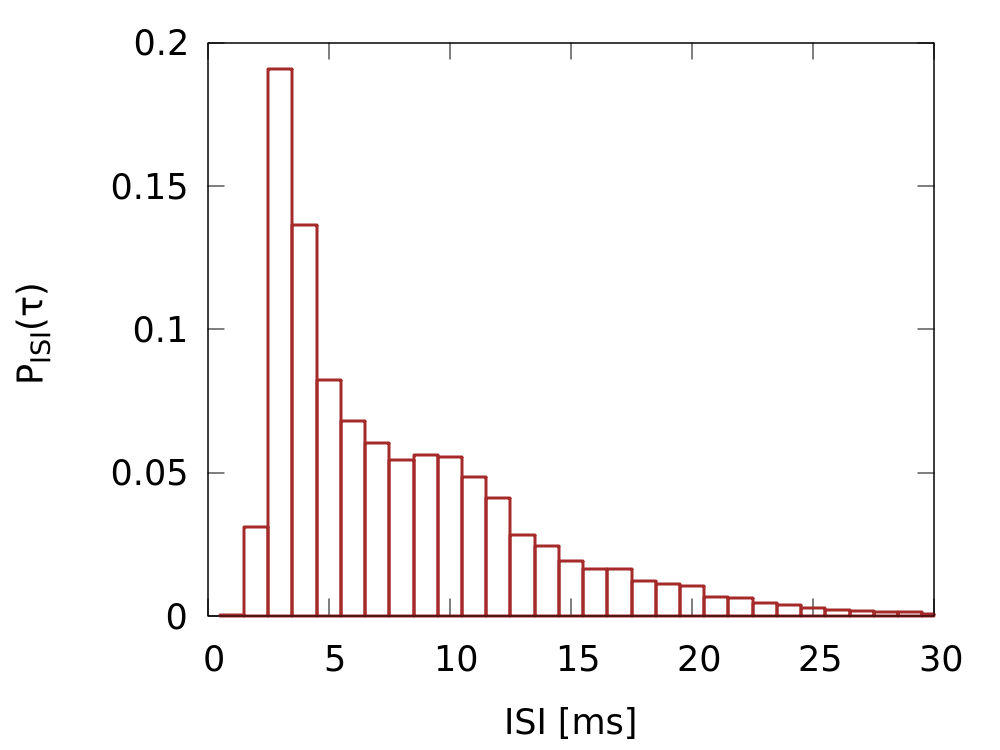
\includegraphics[width=0.45\textwidth]{../Graficos/p_isi.png}
	\caption{Distribución de probabilidad de los valores del ISI}
	\label{p_isi}
	\end{figure}

\section*{Distribución de número de spikes \texorpdfstring{$P(N)$}{}}

Se cuentan todos los spikes medidos en cada prueba realizada. De los mismo se calcula el histograma asociado obteniendo la distribución de número de spikes $P(N)$
\begin{figure}[H]
	\centering
	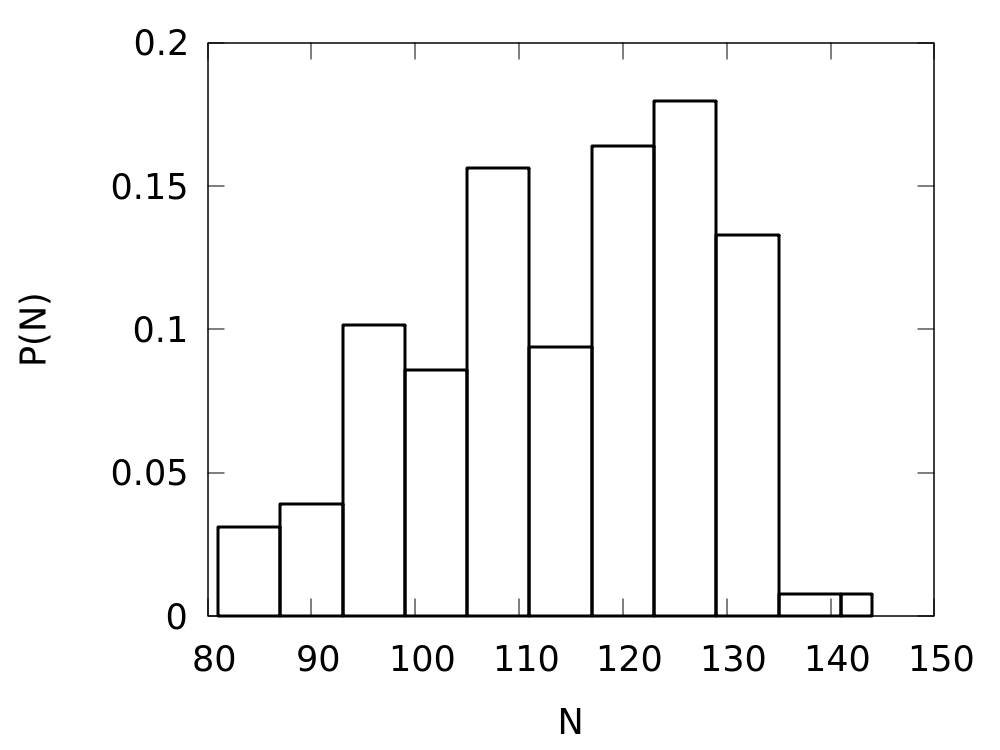
\includegraphics[width=0.45\textwidth]{../Graficos/p_N.png}
	\caption{Distribución de probabilidad de la cantidad de spikes en cada realización del experimento.}
\end{figure}


La distribución tiene una media de $\langle N \rangle = 117.01$ y un varianza de $\sigma^2_{N}=183.195$, mientras que el factor de Fano $F=1.567$.\\

Considerando que los procesos renewal cumplen que $CV=F^2$, en este experimento puede afirmarse que no se trata de un proceso de renewal, es decir que los spikes depende de los spikes anteriores y no solo del anterior.



\section*{Histograma de la tasa de disparo \texorpdfstring{$r(t)$}{}}

Para calcular la tasa de disparo subyacente,  se sumaron todos los spikes medidos en las 128 pruebas en cada ventana de tiempo de medición. Posteriormente, para suavizar la curva, se tomó un intervalo de tiempo $\Delta t = 10\,$ms, en el que se dividió el rango de tiempo de medición y se sumaron todos los spikes en esa venta, para después dividir $\Delta$. Así se calculó los puntos de la Fig.\,\ref{r_t}.


\begin{figure}[H]
	\centering
	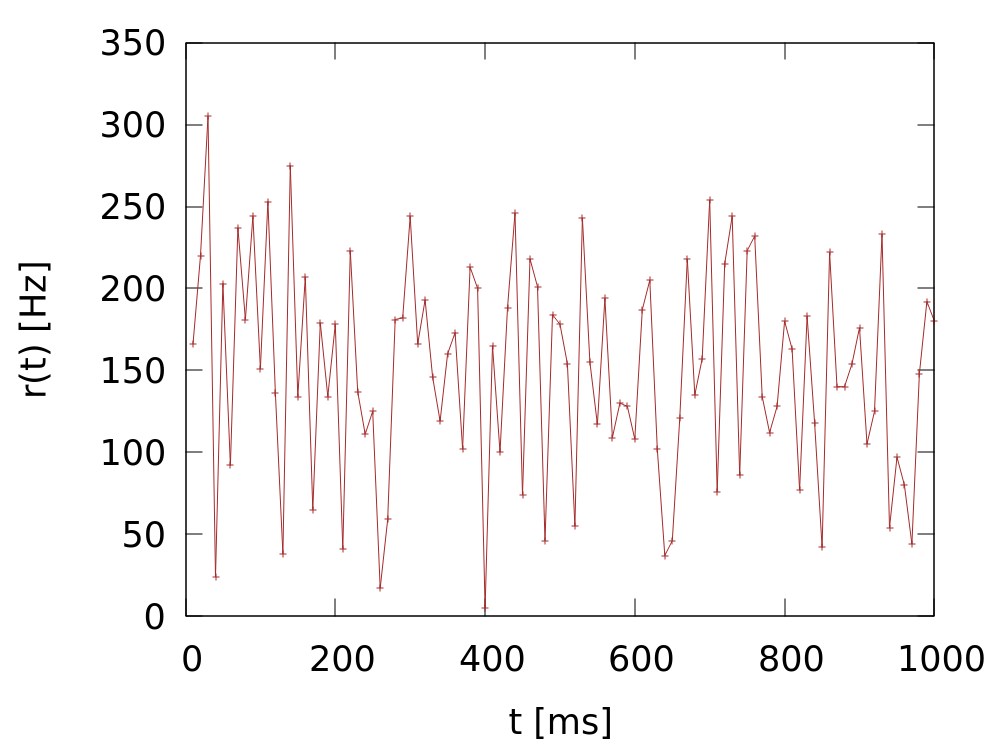
\includegraphics[width=0.45\textwidth]{../Graficos/r_t.png}
	\caption{Tasa de disparo subyacente}
	\label{r_t}
\end{figure}

\section*{Filtro asociado a la neuronas \texorpdfstring{$D(\tau)$}{}}

Considerando que la señal es ruido blanco, es decir que $Q_{s,s}(\tau, \tau')= \sum_{spikes} \sigma^2_s \delta(\tau-\tau')$, se obtiene que el filtro asociado que se  calcula  según las Ec.(\ref{d_t}) y Ec.(\ref{qrs}) 
\begin{align}
    D(\tau) &= \frac{Q_{r,s}(-\tau)}{\sigma^2}, \label{d_t}\\
    \text{  con } Q_{r,s}(-\tau)&= \sum_{spikes} S(t_{spike} - \tau) \label{qrs}
\end{align}
donde $S(t)$ es el valor del estimulo al tiempo $t$

Para calcular la función $D(\tau)$ se implementó  el  algoritmo presentado en el Apéndice \ref{algor}. El mismo recorre un rango de los posibles valores de $-\tau$. Luego para un valor particular $-\tau$, se calcula la suma S($\sum_{spikes} S(t_{spike} - \tau$) sobre los spikes de todas las pruebas, donde en $t_{spike}$ se midió al menos un spike en esa ventana. Los valores de $D(\tau)$ calculados se presentan en en la Fig.\ref{d_tau}. 
\begin{figure}[H]
	\centering
	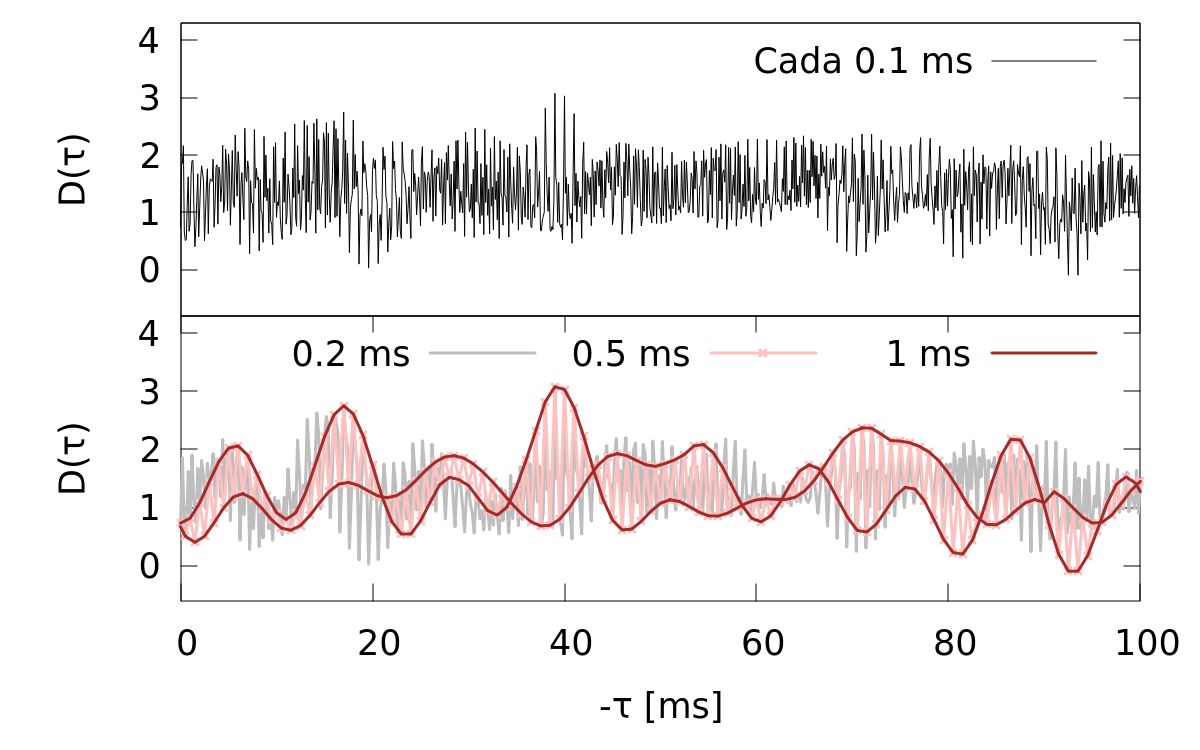
\includegraphics[width=0.5\textwidth]{../Graficos/D_tau.png}
	\caption{La función $D(\tau)$ }
	\label{d_tau}
\end{figure}

\appendix
\section{Algoritmo} \label{algor}

Para calcular la función $D(\tau)$, se implementó  el siguiente algoritmo:

\begin{lstlisting}[language=C++]
int N  		  = 10000;
int N_signal  = 10001;

float var_s  = 31.65;

for (int i = -1000; i < 1000; ++i) //Tau
{
 for (int j = 0; j < N; ++j) //t_spike
 	{ t_evaluate= j+i;
	  
	  if (t_evaluate>=0 
	  && t_evaluate<N) 

	  sum+=vec_signal[t_evaluate]*vec_spikes[j];
	  //Suma sobre todos los spikes en esa ventana
	}
	
	filtro_file<< i <<"\t"<< sum/var_s<<endl;
	sum=0.0;
}
\end{lstlisting}
donde \textbf{vec\_signal} y \textbf{vec\_spikes} son los vectores que contienen a la señal y a la cantidad de spikes de las 128 pruebas en cada ventana de medición, \textbf{N\_signal} y \textbf{N} son las longitudes de \textbf{vec\_signal} y \textbf{vec\_spikes} respectivamente.

\end{document}

